\section{Results}
\subsection{I-V curves} \label{sec:results_iv}
Measures were conducted at temperatures between $(124 \pm 3)$ K and $(296\pm1)$ K. 
The acquired current-voltage curves and their fits from \autoref{eq:iv_curve} are depicted in \autoref{fig:iv-curves}.
The measures fit well with the thermionic emission model throughout the studied range of voltage, with currents of the order of the mA.
The barrier height $\Phi_b$ as a function of temperature, extrapolated from \autoref{eq:iv_curve}, is depicted in \autoref{fig:iv-barrier-height}.
$\Phi_b$ was observed to rise linearly with the temperature, ranging from $(0.20 \pm 0.01)$ eV at $(124 \pm 3)$ K to $(0.50 \pm 0.02)$ eV at $(296 \pm 1)$ K.


\begin{figure}[htbp]
    \centering
    \begin{minipage}[t]{0.49\textwidth}
        \centering
        {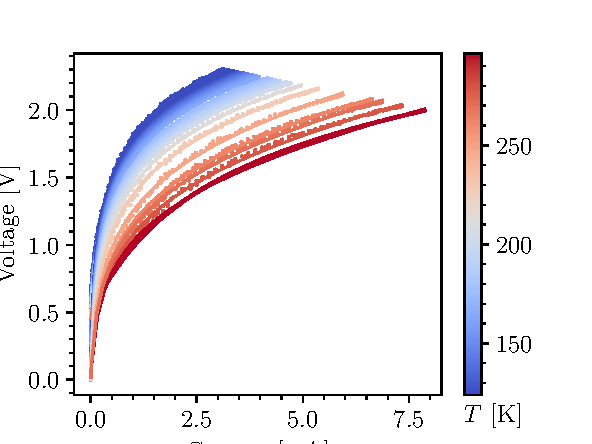
\includegraphics[scale=1]{figures/iv-curves.pdf}}
        \captionsetup{width=.95\linewidth}
        \captionof{figure}{Current-Voltage curves measured over the metal-semiconductor junction at temperatures ranging from $(124 \pm 3)$ K to $(296 \pm 1)$ K and related fits.}
        \label{fig:iv-curves}
    \end{minipage}
    \begin{minipage}[t]{0.49\textwidth}
        \centering
        {
        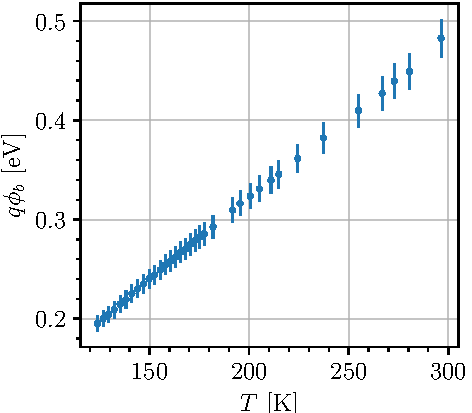
\includegraphics[scale=1]{figures/iv-schottky-potential-temperature.pdf}}
        \captionsetup{width=.95\linewidth}
        \captionof{figure}{Schottky barrier height $\Phi_b$ as a function of temperature as obtained by I-V curves.}
        \label{fig:iv-barrier-height}
    \end{minipage}
\end{figure}

Although this result suggests a dependence in temperature of $\Phi_b$, a study of the barrier height using a Richardson plot was done. Due to the high uncertainty of the ideality factor obtained from the fits, as shown in \autoref{fig:ideality_factor}, the modified Richardson plot method was used. The obtained barrier height from the fit with \autoref{eq:modified_richardson} was found to be $\Phi_b = (1.51 \pm 0.02)$ eV.
\begin{figure}[htbp]
    \centering
    \begin{minipage}[t]{0.49\textwidth}
        \centering
        \captionsetup{width=.95\linewidth}
        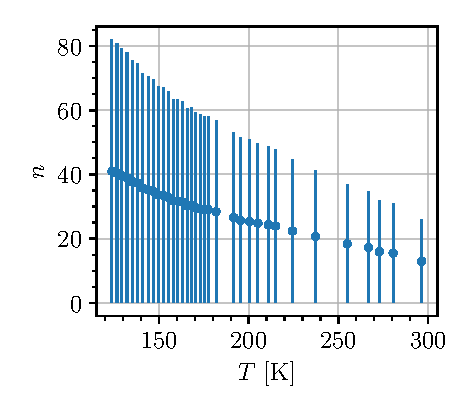
\includegraphics[width=\textwidth]{figures/iv-ideality-factor.pdf}
        \captionof{figure}{Ideality factor $n$ as obtained by the the fits of the $I$-$V$ curves.}
        \label{fig:ideality_factor}
    \end{minipage}
    \begin{minipage}[t]{0.49\textwidth}
        \centering
        \captionsetup{width=.95\linewidth}
        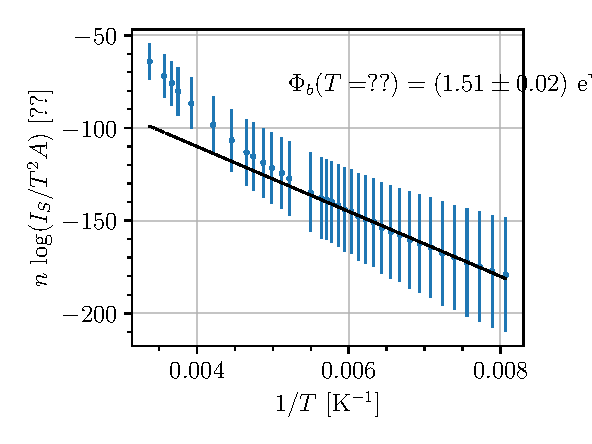
\includegraphics[width=\textwidth]{figures/richardson.pdf}
        \captionof{figure}{Modified Richardson plot.}
        \label{fig:richardson}
    \end{minipage}
\end{figure}

\subsection{Internal photoemission} \label{sec:results_photoemission}
The photocurrent was measured between wavelengths $200$ nm and $1100$ nm.
Due to the unexpected behavior of the filters, not corresponding to their given cutoff wavelength, as shown in \autoref{sec:calibration_curves}, no filter was used for this part of the experiment.
\autoref{fig:photocurrent_curve} shows as an exemple the calibrated spectrum acquired at $T = (100\pm3)$ K.
The linear portion between $1.3$ and $1.8$ eV was identified as the one related to photoemission and thus the fit using \autoref{eq:fowler} was carried out in that range.
The values of $\Phi_b$ obtained in each spectrum by finding the intercept with the $x$ axis are depicted in \autoref{fig:photoemission_phi}.
Contrary to what was found in  \autoref{sec:results_iv}, this method highlighted a barrier height decreasing with increasing temperature.
\begin{figure}[htbp]
    \centering
    % ACHTUNG ACHTUNG ACHTUNG ACHTUNG ACHTUNG: TODO MAYBE NOT USE VSPCAE
    \vspace{-0.2cm}
    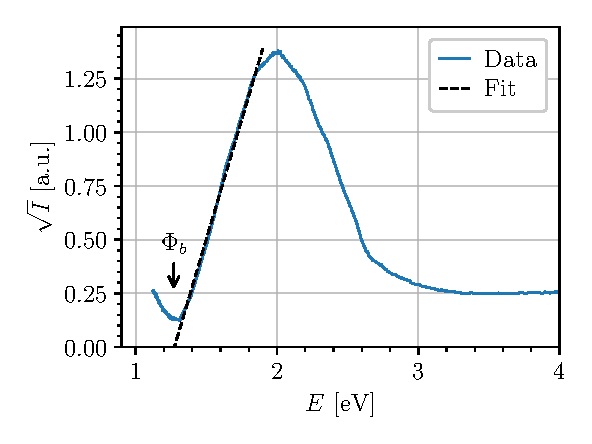
\includegraphics[scale=1]{figures/photocurrent_curve.pdf}
    \caption{Calibrated spectrum of the photocurrent as a function of the incident photon energy $E=h\nu$}
    \label{fig:photocurrent_curve}
    \vspace{-1.5cm}
\end{figure}
\begin{figure}[htbp]
    \centering
    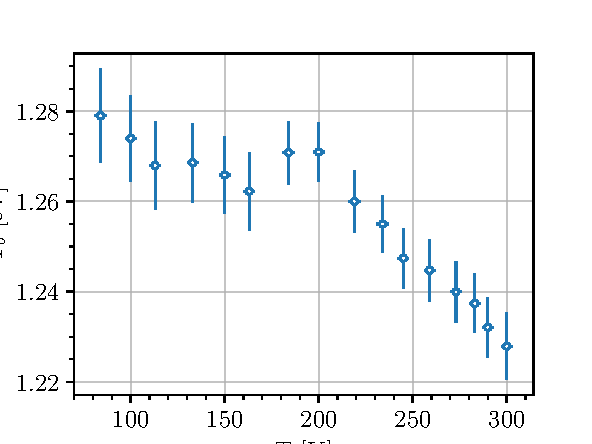
\includegraphics[scale=1]{figures/photoemission_phi.pdf}
    \caption{Schottky barrier height $\Phi_b$ as a function of temperature as obtained by photocurrent measurements.}
    \label{fig:photoemission_phi}
\end{figure}


